\documentclass[xcolor=dvipsnames, 14pt]{beamer} 
\usecolortheme[named=Brown]{structure} 
% \useoutertheme{umbcfootline}
\usetheme[height=10mm]{Rochester} 
% \usetheme{Rochester} 

\setbeamertemplate{items}[default] 
\setbeamertemplate{itemize subitem}[circle] % if you wnat a circle

\usepackage[spanish]{babel}
\usepackage[utf8]{inputenc}

\usepackage{graphicx}

\usepackage{color}
\usepackage{inconsolata}

\usepackage{xcolor}

\usepackage{listings}
% \lstset{ %
% breaklines=true,            % sets automatic line breaking
% frame=single,               % Add a frame to listings.
% basicstyle=\footnotesize,   % Font size.
% }
\lstset{ 
    % language=Prolog,    
    basicstyle=\ttfamily\small, % Usa inconsolata
    identifierstyle=\ttfamily,
    keywordstyle=\color[rgb]{0,0,1},
    commentstyle=\color[rgb]{0.133,0.545,0.133},
    stringstyle=\color[rgb]{0.627,0.126,0.941},
    morekeywords={true,false},
    showstringspaces=false,     % No muestra underscores en los espacios de los strings.
    backgroundcolor=\color{gray!10}, % Un color suave de fondo (menos chocante que el frame=single)
    breaklines=true,            % Wrappea las lineas automáticamente.
    % numbers=left,                    % where to put the line-numbers; possible values are (none, left, right)
    % numbersep=5pt,                   % how far the line-numbers are from the code
    % numberstyle=\tiny\color{gray},
    belowskip=0pt               % Reduce el espacio entre un listing y el párrafo siguiente
    %frame=single               % Un recuadro en los listings.
}

\usepackage[absolute,overlay]{textpos}
\newenvironment{reference}[2]{%
  \begin{textblock*}{\textwidth}(#1,#2)
      \footnotesize\it\bgroup\color{gray!50!black}}{\egroup\end{textblock*}}
% 128mm×96mm

% items enclosed in square brackets are optional; explanation below
\title{Invisble.js}
\subtitle{Trabajo profesional de Ingeniería en Informática}
\author{
Martín Paulucci \\
Facundo Olano
}
\institute[UMBC]{
  Facultad de Ingeniería\\
  Universidad de Buenos Aires \\
}
\date{20 de Diciembre, 2013}

\newtheorem{codigo}{Código}

\begin{document}

%--- the titlepage frame -------------------------%
\begin{frame}[plain]
  \titlepage
\end{frame}

\begin{frame}{Arquitectura Web}
    \begin{center}
        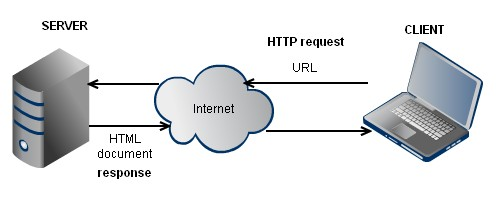
\includegraphics[width=\textwidth]{img/http.png}
    \end{center}
\end{frame}


\begin{frame}{Programación Web: Prehistoria}
    \begin{columns}[c]
        \begin{column}{0.5\textwidth}
            \begin{itemize}
                \item Páginas estáticas
                \item CGI Scripts
                \item Aplicaciones tradicionales (Java, PHP)
            \end{itemize}
        \end{column}
        \begin{column}{0.5\textwidth}
            \begin{center}
                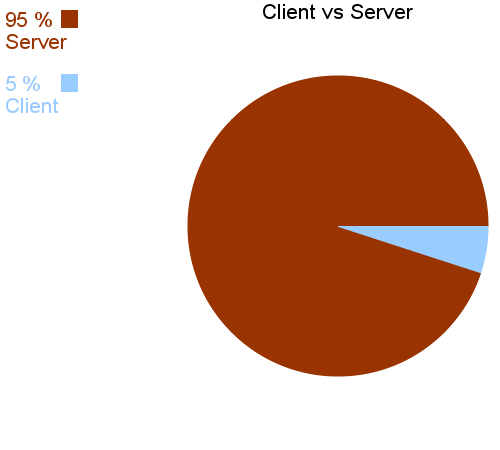
\includegraphics[width=\textwidth]{img/prehistoria2.png}
            \end{center}
        \end{column}
    \end{columns}
\end{frame}


\begin{frame}{Programación Web: Historia}
    \begin{columns}[c]
        \begin{column}{0.5\textwidth}
            \begin{center}
                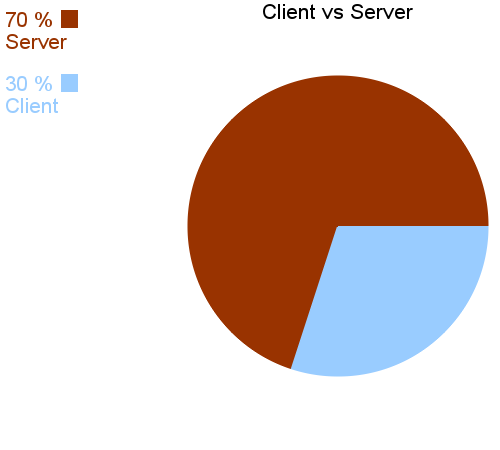
\includegraphics[width=\textwidth]{img/historia2.png}
            \end{center}
        \end{column}
        \begin{column}{0.5\textwidth}
            \begin{itemize}
                \item Frameworks MVC (Rails, Django, Cake)
                \item Interfaces amigables (JavaScript)
                \item Interfaces dinámicas (JQuery, AJAX)
            \end{itemize}
        \end{column}
    \end{columns}

\end{frame}

\begin{frame}{Programación Web: Actualidad}

\begin{columns}[c]
    \begin{column}{0.5\textwidth}
        \begin{itemize}
            \item HTML5, Realtime
            \item Backbone
            \item MVVM: Knockout, Angular
        \end{itemize}
    \end{column}
    \begin{column}{0.5\textwidth}
        \begin{center}
            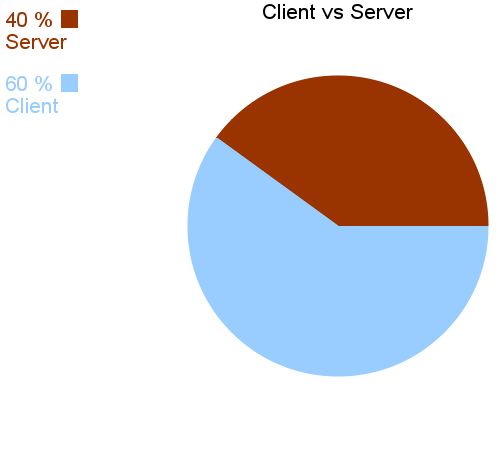
\includegraphics[width=\textwidth]{img/actualidad2.png}
        \end{center}
    \end{column}
\end{columns}

\end{frame}

\begin{frame}{Problemas Actuales}
\begin{reference}{4mm}{85mm}
``Pocas veces pensamos en lo que tenemos; pero siempre en lo que nos falta.'' Jorge Luis Borges
\end{reference}
    \begin{itemize}
        \item Duplicación de modelos
        \item Duplicación de validaciones
        \item Constante cambio del lenguaje
    \end{itemize}
    \begin{center}
        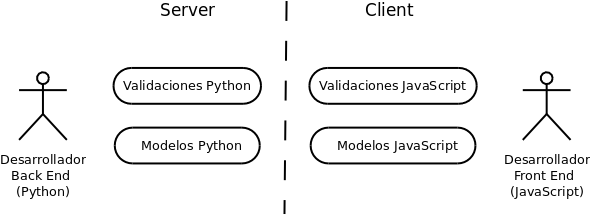
\includegraphics[width=0.8\textwidth]{img/problemas.png}
    \end{center}
\end{frame}

\begin{frame}{Programación Web: Futuro}
\begin{reference}{4mm}{13mm}
``The best way to predict the future is to invent it.'' Alan Kay
\end{reference}

\begin{columns}
    \begin{column}{0.3\textwidth}
        \begin{itemize}
            \item Meteor
            \item Derby
            \item Invisible?
        \end{itemize}
    \end{column}
    \begin{column}{0.7\textwidth}
        \begin{center}
            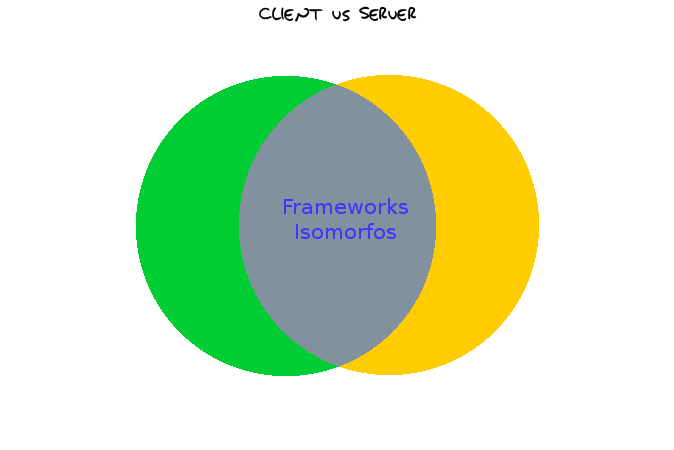
\includegraphics[width=\textwidth]{img/futuro.png}
        \end{center}
    \end{column}
\end{columns}

\end{frame}

\begin{frame}{Nuestro objetivo}
\begin{reference}{4mm}{85mm}
``Al buscar lo imposible el hombre siempre ha realizado y reconocido lo posible.'' Mijaíl Bakunin
\end{reference}

\begin{itemize}
    \item Definir modelos una vez, utilizarlos en cualquier lugar
    \item Validaciones definidas una vez
    \item Métodos CRUD utilizados indistintamente en servidor y cliente
    \item Soporte Realtime
\end{itemize}

\end{frame}

\begin{frame}{Investigación}
\begin{reference}{4mm}{13mm}
``If you think it's simple, then you have misunderstood the problem.'' Bjarne Stroustrup
\end{reference}

\begin{columns}

\begin{column}{0.5\textwidth}
    \begin{itemize}
    \item CoffeeScript
    \item Server Push
        \begin{itemize}
        \item Log Polling
        \item SSE
        \item WebSockets
        \item socket.io
        \end{itemize}
    \item REST
    \item Templates
    \end{itemize}
\end{column}

\begin{column}{0.5\textwidth}
    \begin{itemize}
    \item node.js
        \begin{itemize}
        \item Express
        \item Derby
        \item Meteor
        \item Flatiron
        \end{itemize}
    \item Client MV*
        \begin{itemize}
        \item Backbone
        \item Angular
        \item Knockout
        \end{itemize}
    \end{itemize}
\end{column}

\end{columns}

\end{frame}

\begin{frame}{Prototipos Realizados}
\begin{reference}{4mm}{85mm}
``Hay que unir lo teórico a lo Real, lo ideal a lo Empírico.'' Juan Perón
\end{reference}

\begin{itemize}
    \item \emph Fodder : REST + SSE + Handlebars
    \item \emph drymodels : Node.js + Express + Backbone
    \item \emph Acekia : Node.js + Angular + CoffeeScript
\end{itemize}
\end{frame}

\begin{frame}{Arquitectura en Invisible.js}
\begin{reference}{4mm}{85mm}
``There's only one trick in software, and that is using a piece of software that's already been written.'' Bill Gates
\end{reference}

\begin{center}
    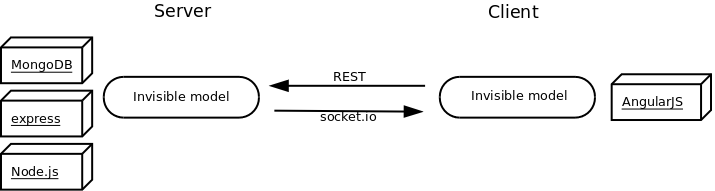
\includegraphics[width=\textwidth]{img/arq.png}
\end{center}


\end{frame}

\begin{frame}[fragile]{Modelos en Invisible.js}

\begin{columns}[t]

\begin{column}{0.5\textwidth}
\begin{lstlisting}
class Person
    getFullName()
    getAvatarUrl()
\end{lstlisting}
\end{column}

\begin{column}{0.5\textwidth}
\begin{lstlisting}
class Person
    getFullName()
    getAvatarUrl()

    save(cb)
    delete(cb)
    query(query, opts, cb)
    findById(id, cb)

    onNew(cb)
    onUpdate(cb)
    onDelete(cb)
\end{lstlisting}
\end{column}
\end{columns}
\end{frame}

\begin{frame}{Modelos en Invisible.js (2)}
    \begin{center}
        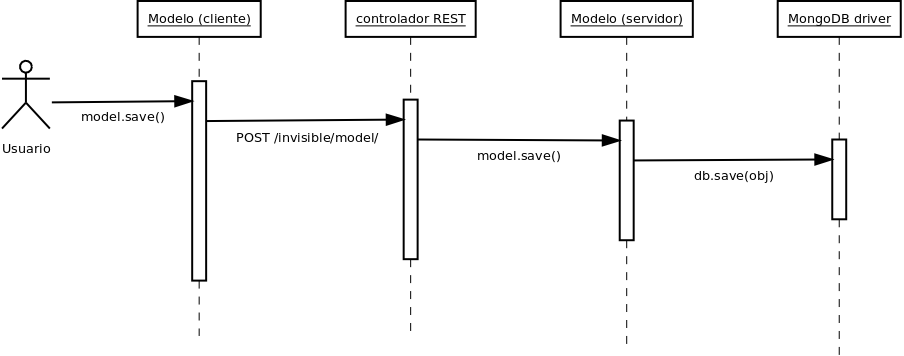
\includegraphics[width=\textwidth]{img/secuencia.png}
    \end{center}
\end{frame}

\begin{frame}[fragile]{Invisible.js en acción: Mensaje}
\begin{reference}{4mm}{13mm}
``Talk is cheap. Show me the code.'' Linus Torvalds
\end{reference}

\texttt{models/message.coffee:}
\begin{lstlisting}
Invisible = require("invisible")

class Message
    constructor: (@from, @body) ->
      @date = new Date()

module.exports = Invisible.createModel("Message", Message)
\end{lstlisting}

\end{frame}

\begin{frame}[fragile]{Invisible.js en acción: Usuario}
\texttt{models/user.coffee:}
\begin{lstlisting}
crypto = require("crypto")

SALT = "MY REALLY LONG HASH SALT"

class User
    constructor: (@email)->

    setPassword: (plainPassword) ->
        h = crypto.createHash('sha1')
        h.update(plainPassword)
        h.update(SALT)
        @password = h.digest('base64')
\end{lstlisting}
\end{frame}

\begin{frame}[fragile]{Invisible.js en acción: Validaciones}
\begin{reference}{4mm}{13mm}
``Programming is usually taught by examples.'' Niklaus Wirth
\end{reference}

\texttt{models/user.coffee:}
\begin{lstlisting}
validations: { methods: ['checkUnique'] }

checkUnique: (done) ->
    Invisible.User.query {email: @email}, (err, res) ->
        if res.length == 1
            done({valid : false, errors: ["email already registered"]})
        else if res.length == 0
            done({valid : true})
\end{lstlisting}
\end{frame}

\begin{frame}[fragile]{Invisible.js en acción: Configuración}
\texttt{app.coffee:}
\begin{lstlisting}
invisible = require("invisible")
express = require("express")
app = express()

# Express middleware

invisible.createServer app, "models", () ->
  console.log("Invisible server listening on port " + app.get("port"))
\end{lstlisting}
\end{frame}

\begin{frame}[fragile]{Invisible.js en acción: Configuración (2)}
\texttt{public/index.html:}
\begin{lstlisting}[language=html]
<html>
    <body>
        <script src="invisible.js"></script>
        <script type="text/javascript">
            var message = new Invisible.Message()
            console.log(message.date)
        </script>
    </body>
</html>
\end{lstlisting}
\end{frame}

\begin{frame}{Demo}
    \begin{center}
        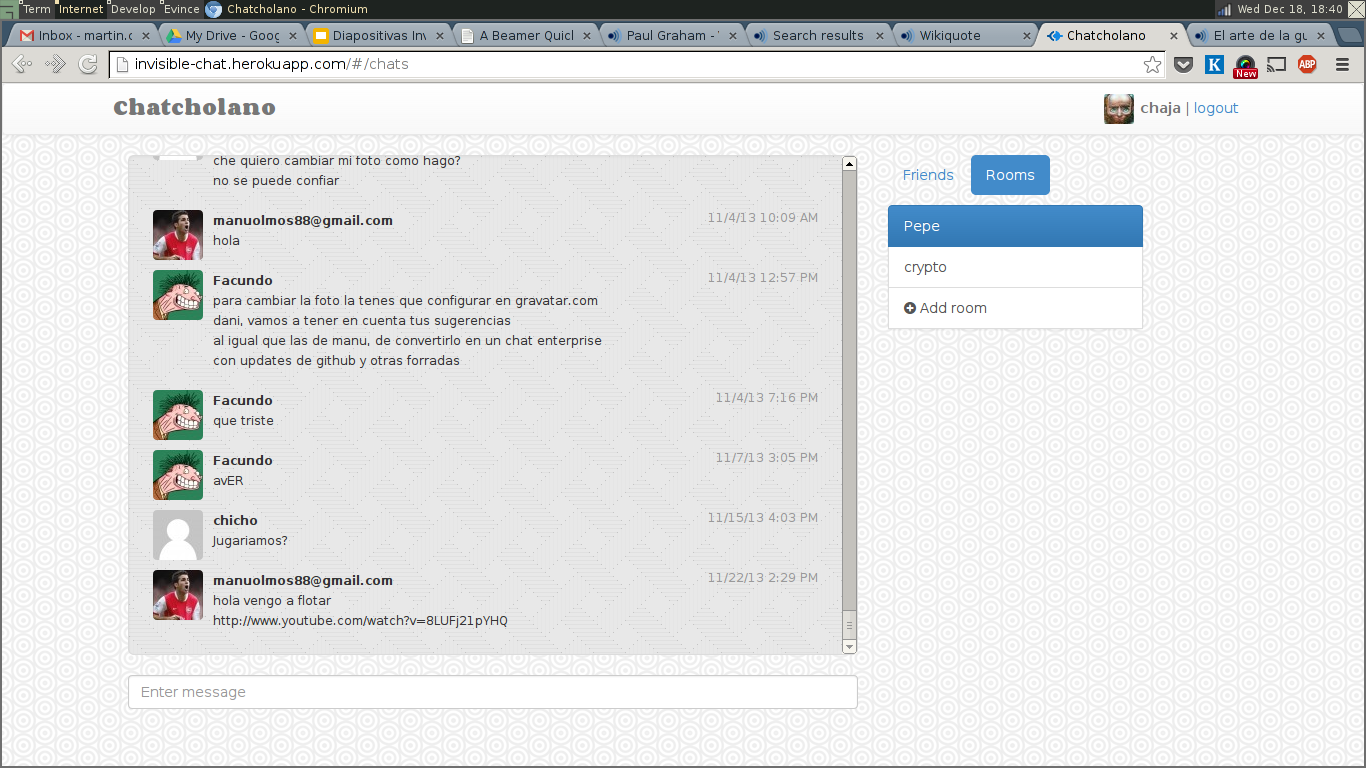
\includegraphics[width=\textwidth]{img/demo.png}
    \end{center}
\end{frame}

\begin{frame}{Conclusiones}
\begin{itemize}
    \item Se realizó un trabajo integral de Ingeniería de Software.
    \item Se obtuvo un framework útil, sencillo de utilizar, y con potencial de desarrollo.
    \item Se cumplieron los objetivos del proyecto y se superaron las expectativas iniciales.
\end{itemize}
\end{frame}

\begin{frame}{Repercusiones}
\begin{reference}{4mm}{13mm}
``The secret of politics? Make a good treaty with Russia.'' Otto von Bismarck
\end{reference}

\begin{columns}[t]

\begin{column}{0.5\textwidth}
    \begin{center}
        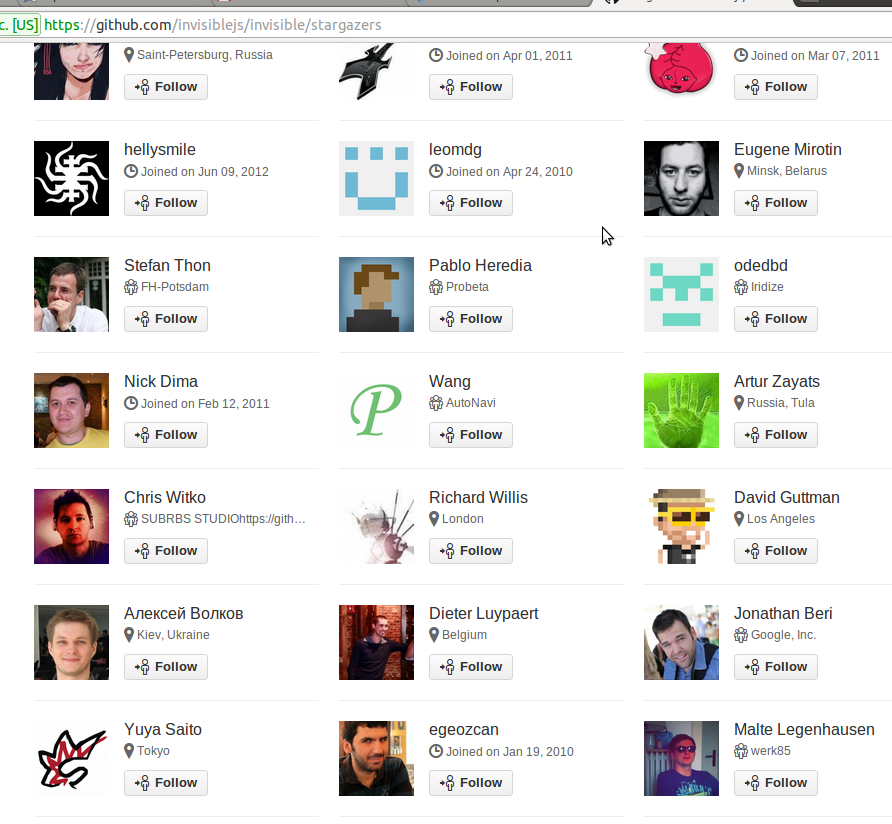
\includegraphics[width=\textwidth]{img/github.png}
    \end{center}
\end{column}

\begin{column}{0.5\textwidth}
    \begin{center}
        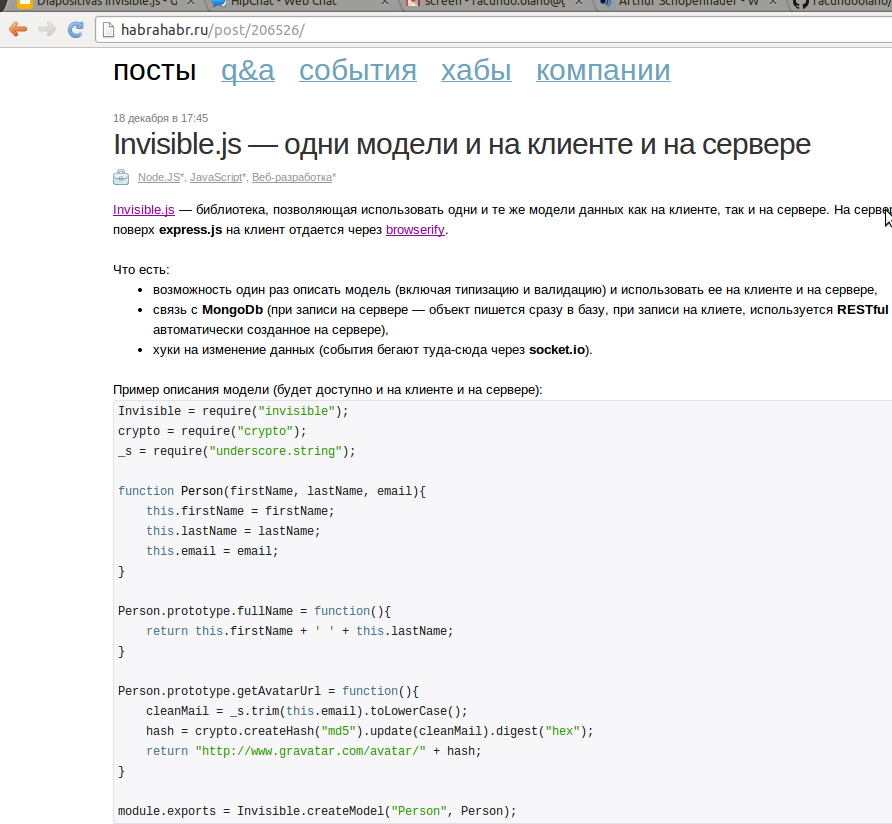
\includegraphics[width=\textwidth]{img/rusia.png}
    \end{center}
\end{column}
\end{columns}


\end{frame}

\begin{frame}{Trabajo futuro}
\begin{itemize}
    \item Implementar módulo de seguridad
    \item Evaluar escalabilidad
    \item Incentivar el desarrollo comunitario
\end{itemize}

\end{frame}

\begin{frame}[c]{Preguntas}
% \begin{reference}{4mm}{13mm}
% ``El artista es el ingeniero del alma humana.'' Iósif Stalin
% \end{reference}
\Huge Preguntas?
\end{frame}

% cd

\end{document}
